\documentclass{article}
\usepackage[T1]{fontenc}
\usepackage{titling}
\setlength{\droptitle}{-10em}
\title{Project Part 2 Writeup}
\author{Sasha Yousefi}
\usepackage{algorithm2e}
\RestyleAlgo{ruled}
\usepackage{amsmath}
\usepackage{graphicx}
\usepackage{caption}
\usepackage{subcaption}
\usepackage[section]{placeins}
\begin{document}
\maketitle
\section{Introduction}
In this project, we developed a program to solve the steady state heat equation in C++. We consider the scenario where we are transferring hot fluid within a pipe (temp $T_h$) and using an exterior series of cold jets (temp $T_c$) to keep the outer portion of the pipe cool. We then use our implemented algorithm to find the mean temperature within the pipe walls. The solution domain for our system is discretized into a series of grid points and boundary conditions at exposed surfaces. Each interior position is replaced with a finite difference approximation, which are used to construct linear equations for each point. Using this mathematical interpretation, we are able to set up and solve a system of linear equations (-A)u = b using the iterative Conjugate Gradient (CG) method. The CG. Since CG only requires matrix-vector products, it is quite an efficient iterative method to solve linear systems when the matrix "A" is sparse.\cite{CME211:2021:FinalProjectPart1}\cite{CME211:2021:FinalProjectPart2}
\section{CG Solver Implementation}
To implement our CG Solver, we utilize object oriented programming in C++. First, we create a SparseMatrix class, which defines a sparse matrix object that contains the appropriate methods and variables to build a system of linear equations. We then define a HeatEquation2d class, which sets up and solves our linear system. To set up our SparseMatrix object, A, we treat each row of the matrix as an equation for a particular point on the discretized grid. We build our matrix by calling methods in the SparseMatrix class, which implement our matrix in COO format. We simultaneous build our solution vector (the right hand side "b" of our linear system) while building the matrix, This vector contains a zero element at the interior node positions and a heat boundary value, $T_c$ or $T_h$, at the exterior boundary positions. In order to handle the edge case that there is only one row, we add to our solution vector additively so that both boundary positions are added to the right hand side of the equation. Lastly, we set our initial guesses for "u" as all zeros. 

After converting the matrix to CSR format by calling the appropriate function within our SparseMatrix class, we are able to solve the system of linear equations using the CG method outlined below. This method takes in a SparseMatrix object, a solution vector, an initial guess vector, and a tolerance, and solves our linear system by iteratively approximating the solution. The CGSolver displays OOP by taking in an object and calling the object's method in order to calculate matrix-vector products. Additionally, the CGSolver computes vector operations (such as finding the L2 norm, vector-scalar multiplication, vector addition, and vector-vector multiplication) using a helper file, MatVecOps. To avoid extraneous copying, we pass our SparseMatrix object and solution vector by reference into the CGSolver algorithm. \cite{CME211:2021:FinalProjectPart2}
\SetKwComment{Comment}{/* }{ */}
\begin{center}
\begin{algorithm}[H]
\SetAlgoLined
\caption{CG Algorithm}\label{alg:two}
initialize $u_0$\;
$r_0$ = $b$ – $Au_0$\;
$L2norm0$ = $L2norm0(r_0)$\;
$p_0 = r_0$\;
$niter$ = 0\;
\While {$niter$ $<$ $nitermax$} {
    $niter$ = $niter$ + 1\;
    $alpha_n$ = $(r_n^{T} r_n)$ / $(p_n^{T}Ap_n)$\;
    $u_{n+1}$ = $u_n$ + $alpha_n p_n$\;
    $r_{n+1}$ = $r_n$ - $alpha_n Ap_n$\;
    $L2normr$ = $L2norm(r_{n+1})$\;
    \If {$L2normr/L2normr0$ $<$ $threshold$} {
        break\;
    }
    $beta_n$ = $(r_{n+1}^{T} r_{n+1})$ / $(r_n^{T} r_n)$\;
    $p_{n+1}$ = $r_{n+1}$ + $beta_np_n$\;
}
\end{algorithm}
\end{center}
\section{User Guide}
\begin{enumerate}
    \item Begin by running the \underline{\emph{make}} command on the command line to compile the most recent version of the program.
    \item Run \underline{\emph{./main [input file] [solution prefix]}} to solve the steady state system with parameters give in the input file. Parameters given are the following: system length, system width, system grid spacing, $T_h$ at the hot boundary and $T_c$ at the cold boundary.
    \item Run \underline{\emph{python3 postprocess.py [input file] [solution file]}} to do the following: plot a psuedocolor plot of the temperature distribution within the pipe wall, compute and overlay the mean temperature isoline, and report the mean temperature in the pipe wall.
    \item Download created images which will be named solution***plot.png from rice and visualize the distributions. The *** will be replaced by numerical values corresponding to the iteration number.
\end{enumerate}

\section{Example Visualizations from Post Processing}
\begin{figure}[!htb]
\vspace*{-4cm}
\centering
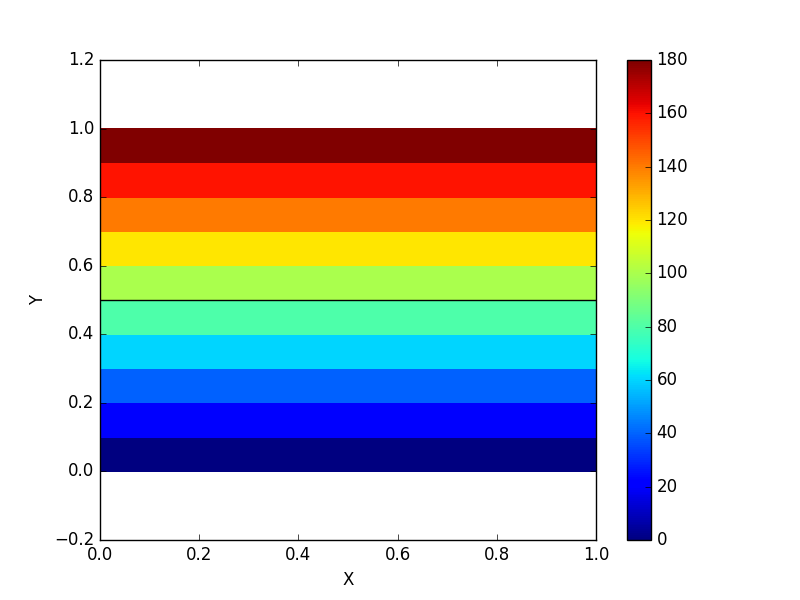
\includegraphics[scale=0.5]{solution009plot.png}
\captionof{figure}{Plot for Input 0}
\label{fig:plot0}
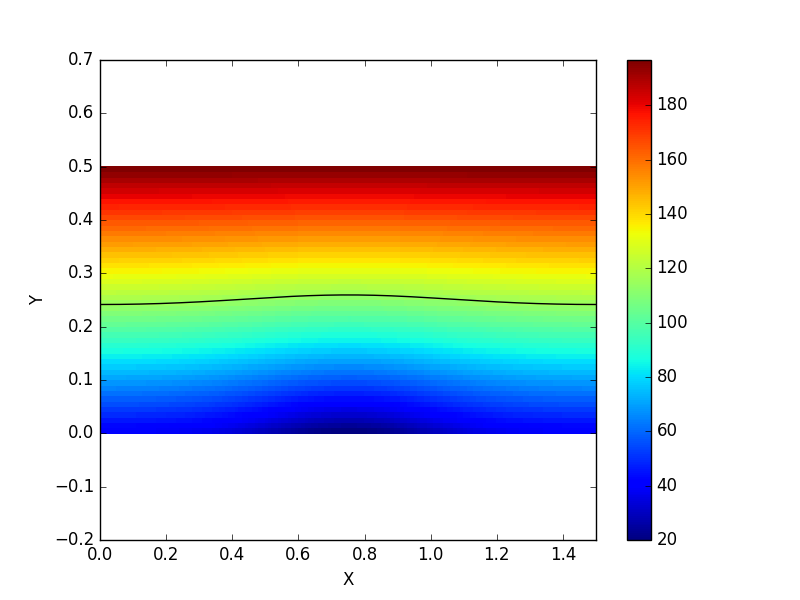
\includegraphics[scale=0.5]{solution132plot.png}
\captionof{figure}{Plot for Input 1}
\label{fig:plot1}
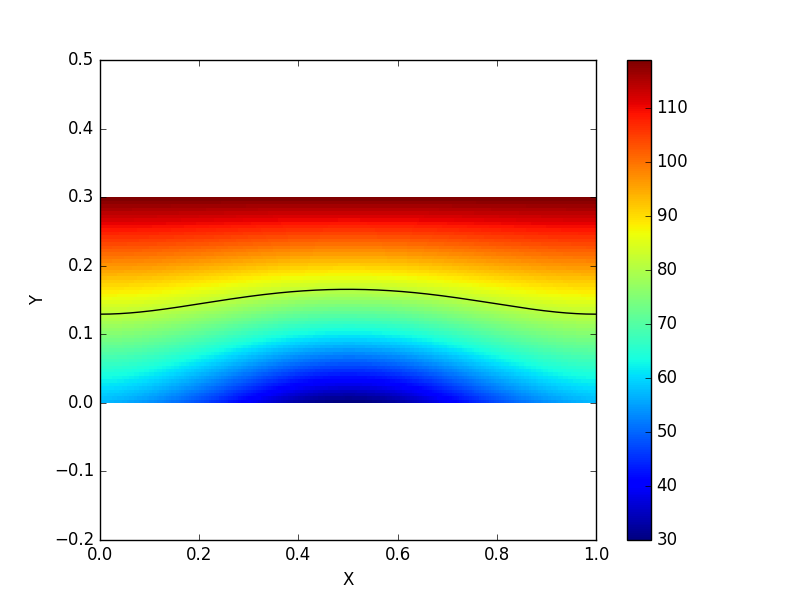
\includegraphics[scale=0.5]{solution157plot.png}
\captionof{figure}{Plot for Input 2}
\label{fig:plot2}
\end{figure}

\bibliographystyle{unsrt}
\bibliography{references}
\end{document}
